This example was designed to introduce \bioptim's ability to reduce the number of degrees-of-freedom (DoF) of a model via the \texttt{mappings}, to account for nonlinear boundaries on the controls, and to solve complex multiphase programs including impacts and free time phases.

We used a full-body model consisting of 3~DoFs at the pelvis (forward and upward translations, tranverse rotation), 1~DoF at each upper limb (shoulder flexion), and 3~DoFs at each lower limb (hip, knee and ankle flexion) for a total of 11 DoFs.
For this optimization, the \texttt{BidirectionalMapping} was used to symmetrize the left-hand side with the right-hand side, effectively creating a 7-DoFs pseudo-2D model. 
Since this is a full-body model, the root segment (i.e., the pelvis) was left uncontrolled, reducing the number of control variables to 4, namely the shoulder, hip, knee and ankle flexions. 

A total of five phases were used to describe the dynamics of the jump, flight and landing. 
The first two were push-off phases consisting in one phase with two ground contacts (heel and toe) and a second one with one contact (toe). 
A contact is described as a point where forces are applied to cancel its acceleration. 
The third phase was purely aerial, described by a free-fall dynamics.
The last two were landing phases, a first one with one contact (toe) and a second one with two contacts (heel and toe).
The transitions between phases with addition of contact points were approximated with the build-in inelastic impact \texttt{PhaseTransition.IMPACT}, which computes the velocity of the kinematic chain after an impact.

The objective function with the most important weight was a Mayer objective computed at the end of the push-off phase consisting in maximizing the jump height ($h$)---represented by the position of the CoM---from the projectile equations.
The remaining objective functions were added either to help the solver to converge (regularization) or to converge toward a more human-like solution. 

\[ 
\resizebox{0.90\columnwidth}{!}{$ 
\begin{aligned}
\mathcal{J} = &~\underbrace{\omega_h h}_{\mathtt{MIN\_PREDICTED\_COM\_HEIGHT}}~+~\underbrace{\omega_{x} \| \mathbf{x}_+(T_5) - \mathbf{x}_+^*\|^2}_{\mathtt{TRACK\_STATE}}\\
+~&\sum^5_{i=1}~\underbrace{\omega_{t}(T_i - T_{i-1})}_{\mathtt{MIN\_TIME}}~
  +~\sum_{i=2}^4\int_{t=T_i}^{T_{i+1}}\underbrace{\omega_{sd}\left|\left|\frac{d\mathbf{\dot{q}}}{dt}\right|\right|^2}_{\mathtt{MIN\_STATE\_DERIVATIVE}}~dt
\end{aligned}  
$} 
\addtag  
\label{eq:cost_jumper}
\]

where $T_0=0$, $T_i$ with $i \in [1, 2, 3, 4, 5]$ are the final times of the i$^{th}$ phase respectively; 
$\omega_h$ is the weight of the maximization of the CoM height and is defined negative ($-100$) to effectively maximize this term objective function; 
$\omega_t$, $\omega_{sd}$ and $\omega_x$ are weights equal to $0.1$, $0.1$, and $1$, respectively; 
$\mathbf{\dot{q}}$ is the generalized velocities part of the state vector $\mathbf{x}$; 
and $\mathbf{x}_+$ is the state vector excluding the translations of the root segment. 
The $\mathbf{x}_+^*$ corresponds to a reference static position of the avatar with its knee slightly flexed and its arms horizontally raised.



Several constraints are necessary to describe a realistic jump.
%The generalized coordinates---i.e., the maximum flexibility expected---are bounded to human-like limits.
Joint angles were bounded to human-like limits.
The first node of the first phase was enforced to be equal to $\mathbf{x^*}$ (i.e., including the translations of the root segment to be at the origin). 
Joint velocities were arbitrarily bounded to $[-10 \pi; 10 \pi]~rad/s$.
Joint torques were bounded with nonlinear torque/angle/velocity relashionships measured on a high level athlete using an isokinetic dynamometer (Fig.~\ref{fig:graph_force_vitesse_longueur}). 
%For the contact forces from the contact points, a directional constraint is applied such that the force is alway pointing upward, meaning that the model is not allowed to pull on the floor. 
%The lateral force norm is constrained to be below the half of the upward force, i.e., the model must remain in a cone of friction more or less corresponding to a show contacting a normal surface. 
Non slipping (\texttt{NON\_SLIPPING}) and unilateral (\texttt{CONTACT\_FORCE}) contact force constraints were added to prevent the contact points from slipping and pulling on the ground.
%Finally, some constraints were added to prevent the gradient descending solver from exploring non interesting regions. 
Finally, some constraints were added to help convergence.
First, during the push-off and landing phases, the heels had to remain over the floor.
Then, the center of mass velocity had to point upward when leaving the floor and at the same instant, the arms had to be frontward. 

\begin{figure}[h!]
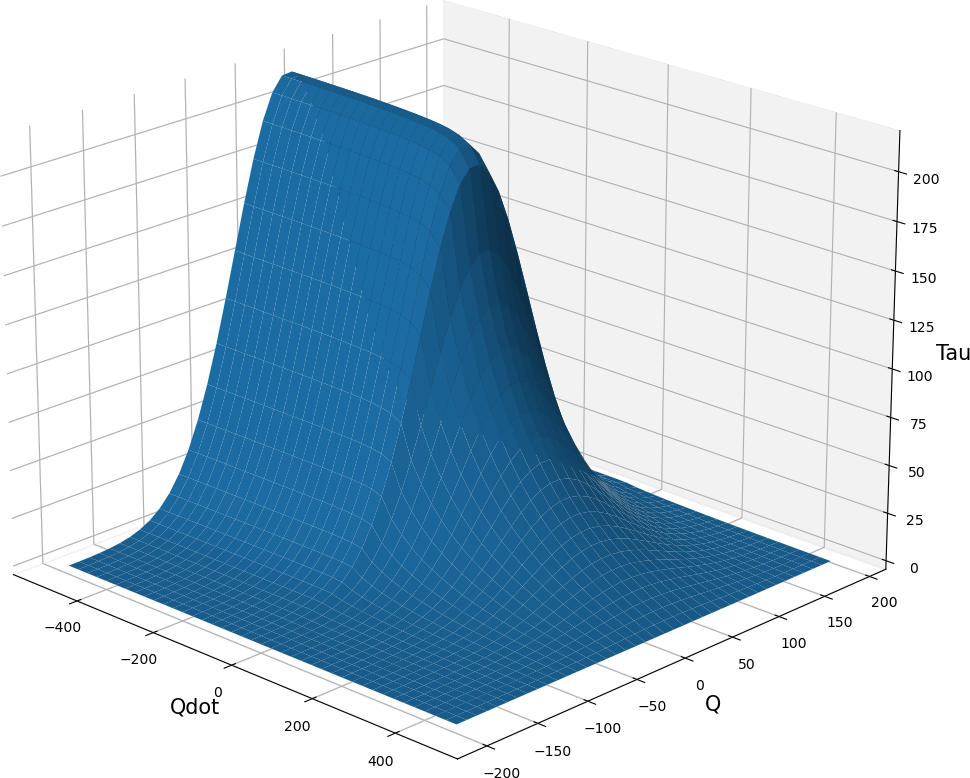
\includegraphics[width=\columnwidth]{figures/torque_angle_velocity_hip_flexion}
\caption{Surface representing the nonlinear constraint from the torque/position/velocity relashionship of the hip flexion} 
\label{fig:graph_force_vitesse_longueur}
\end{figure}

To speed-up the solving of the problem with \emph{ipopt}, the problem was first approximately solved using the BFGS hessian approximation option for 200 iterations maximum.
Then, starting from this first solution, the problem was re-optimized, with exact-hessian computations for up to 1000 iterations.
The optimized solution was obtained in 148 iterations of the exact-hessian optimization for a total optimization time of \SI{1780}{\second} ($\approx\SI{30}{\minute}$), resulting in a \SI{1.28}{\meter} jump height.
The optimized time for the phases $1$ to $5$ were $0.70, 0.05, 0.99, 0.36, 0.21$ seconds, respectively.
The solution reproduced a human proximo-distal strategy (Fig~\ref{fig:graph_force_vitesse_longueur}), i.e., activating large segments first (for instance the torso) and sequentially adding more distal segments, consequently ending up with the ankles.


